% Template for ICASSP-2018 paper; to be used with:
%          spconf.sty  - ICASSP/ICIP LaTeX style file, and
%          IEEEbib.bst - IEEE bibliography style file.
% --------------------------------------------------------------------------
\documentclass{article}
\usepackage{spconf}

% to compile a camera-ready version, add the [final] option, e.g.:
% \usepackage[final]{nips_2017}

\usepackage[utf8]{inputenc} % allow utf-8 input
\usepackage[T1]{fontenc}    % use 8-bit T1 fonts
\usepackage{hyperref}       % hyperlinks
\usepackage{url}            % simple URL typesetting
\usepackage{booktabs}       % professional-quality tables
\usepackage{amsfonts}       % blackboard math symbols
\usepackage{nicefrac}       % compact symbols for 1/2, etc.
\usepackage{microtype}      % microtypography
% set imports
\usepackage{nccmath}        % decrease equation font size
\usepackage{ntheorem}       % theorem writing
\usepackage{cleveref}       % clever references
\usepackage{graphicx}       % for images
\usepackage[table,xcdraw]{xcolor} % for tables
\usepackage{amsmath, amssymb}  % math
\usepackage{bm}                % ?
\usepackage{subcaption}        % images
\usepackage{hyperref}          % linked refs
\usepackage{tikz}   % for graphs
\usetikzlibrary{calc,intersections,through,scopes,arrows,decorations,backgrounds,positioning,fit,petri,automata,shapes}
\tikzstyle{box} = [draw, rectangle, rounded corners, thick, node distance=4em,
text width=3em, text centered, minimum height=3em]
\tikzstyle{container} = [draw, rectangle, dashed, inner sep=2em]
\tikzstyle{line} = [->, thick, -latex']


% set paths
\graphicspath{{./fig/}}

\title{Attacking Speaker Recognition with \\Deep Generative Models}
\name{Wilson Cai, Anish Doshi, Rafael Valle}
\address{UC Berkeley}

\begin{document}
\maketitle
\begin{abstract}
    In this paper we investigate the ability of generative adversarial networks
    (GANs) to synthesize spoofing attacks on modern speaker recognition systems.
    We first show that samples generated with SampleRNN and WaveNet are
    unable to fool a CNN-based speaker recognition system. We propose  a
    modification of the Wasserstein GAN objective function to make use of data
    that is real but not from the class being learned. Our semi-supervised
    learning method is able to perform both targeted and untargeted attacks,
    raising questions related to security in speaker authentication systems. 
\end{abstract}

\section{INTRODUCTION} \label{sec:introduction}
Speaker recognition and authentication systems are being deployed for security
critical applications such as banking, forensics, home automation, etc. Like
other domains, these systems benefit from recent advancements in deep
learning that lead to improved accuracy and trainability of such systems.
Despite the improvement in the efficiency of these systems, evidence shows that
they can be suspectible to adversarial attacks\cite{wu2015spoofing}, thus motivating a current trend
focused understanding adversarial attacks (\cite{szegedy2013intriguing}, \cite{goodfellow2014explaining}) and finding countermeasures to detect of deflect them. 

Parallel to these advancements, neural speech \textit{generation} (the process of using deep neural networks to generate human-sounding speech) has also seen huge progress (\cite{wang2017tacotron}, \cite{arik2017deep}). Generative Adversarial Networks (GANs) have recently been found to produce incredibly  authentic samples in a variety of fields. The core idea of GANs - namely the minimax game played between a generator network and a discriminator network - extends very naturally to the field of speaker authentication and spoofing. \\
The combination of these advancements begs a natural question that has, to the
best of our knowledge, not been answered:
\begin{center}
Are state-of-the-art speech recognition systems robust \\to adversarial attacks by speech generative models?
\end{center}

More specifically, we contemplate this question and offer in this paper the following contributions:
\begin{itemize}
\item We evaluate SampleRNN and WaveNet in their ability to fool text-independent state-of-the-art speaker recognizers.
\item We propose strategies for untargeted attacks using Generative Adversarial Networks.
\item We propose strategies for targeted attacks using a new objective function based on the improved Wasserstein GAN.
\end{itemize}

%
\section{RELATED WORK}\label{sec:related_work}
Modern generative models are sophisticated enough to produce fake\footnote{We use the term fake to refer to
computer generated samples} speech samples that can be indistinguishable from real human speech. Here, we provide a summary of some existing neural speech synthesis models and their architectures.
WaveNet~\cite{van2016wavenet} is a generative neural network that is trained end-to-end
to model quantized audio waveforms. The model is fully
probabilistic and autoregressive, using a stack of causal convolutional layers
to condition the predictive distribution for each audio sample on all previous ones. It has produced impressive results for generation of speech audio conditioned on speaker and text and has become a standard baseline for neural speech generative models. 

SampleRNN~\cite{mehri2016samplernn} is another autoregressive architecture that
has been successfully used to generate both speech and music samples. SampleRNN
uses a hierarchical structure of deep RNNs to model dependencies in the sample
sequence. Each deep RNN operates at a different temporal resolution so as to
model both long term and short term dependencies. 


Recent work on deep learning architectures has also introduced the presence of \textit{adversarial examples}: small perturbations to the original inputs, normally imperceptible to humans, which nevertheless cause the architecture to generate an incorrect or deliberately chosen output. In their brilliant papers, ~\cite{szegedy2013intriguing} and
~\cite{goodfellow2014explaining} analyze the origin of adversarial attacks and
describe simple and very efficient techniques for creating such perturbations, such as the fast gradient sign method. 

In the vision domain, ~\cite{sharif2016accessorize} describe a technique for attacking facial recognition systems. Their attacks are physically realizable and inconspicuous, allowing an attacker to impersonate another individual. In the speech domain,~\cite{carlini2016hidden} describe attacks on speech-recognition systems which use sounds that are hard to recognize by humans but interpreted as specific commands by speech-recognition systems.

To the best of our knowledge, GANs have not been used before for the purpose of speech synthesis. \cite{pascual2017segan} uses a conditional GAN for the purpose of speech \textit{enhancement}, i.e. taking as input a raw speech signal and outputting a denoised waveform. The model in \cite{chang2017learning} tackles the reverse problem of using GANs to learn certain representations given a speech spectrogram. We believe the use of spectrograms is a step in the right direction of GAN speech research, as using the raw waveform as input has highlighted current issues with using GANs with sequential modeling.
%
\section{ATTACKING SPEAKER RECOGNITION MODELS}\label{sec:spk_rec_atks}
\subsection{Neural speaker recognition system}
\label{sub:speaker_recognition}
The speaker recognition system used in our experiments is based on the
framework by \cite{lukic2016speaker} and is described in Figure
\ref{fig:CNN}. The first module at the bottom is a pre-processing step that
extracts the Mel-Spectrogram from the waveform as described in section
\ref{sub:processdata}. The second module is a convolutional neural network (CNN)
that performs multi-speaker classification using the Mel-Spectrogram. The CNN is
a modified version of Alexnet~\cite{krizhevsky2012imagenet}. We warn the readers
that unlike~\cite{lukic2016speaker}, our classifier operates on 64 by 64 Mel-Spectrogram
and has slightly different number of nodes on each layer.

\begin{figure}[!ht]
    \begin{centering}
    \tikzset{ordinary/.style = {rectangle,draw,thick,rounded corners, minimum
        height = 0.5cm, minimum width=5cm, text width=5cm]}}
    \begin{tikzpicture}[node distance=0.8cm, scale=0.52, every
        node/.style={scale=0.52}]
       \node [] at (0,0) (start) {64 x 64 Mel-Spectrogram};
       \node [above=0.2cm of start] (a) {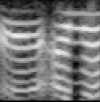
\includegraphics[width=.25\columnwidth]{figures/real_single_mel.png}};
       \node [ordinary,above=0.2cm of a] (b) {L1: convolution \hfill 3x3x32};
       \node [ordinary,above of=b] (c) {L2: max pooling \hfill 2x2};
       \node [ordinary,above of=c] (d) {L3: convolution \hfill 3x3x64};
       \node [ordinary,above of=d] (e) {L4: max pooling \hfill 2x2};
       \node [ordinary,above of=e] (f) {L5: dense \hfill 1024};
       \node [ordinary,above of=f] (g) {L6: dropout \hfill 50\%};
       \node [ordinary,above of=g] (h) {L7: dense \hfill 103};
       \node [ordinary,above of=h] (i) {L8: softmax};
       \node [above=0.2cm of i] (j) {labels};
       \draw[-] (a) -- coordinate (a) (b);
       \draw[-] (b) -- coordinate (b) (c);
       \draw[-] (c) -- coordinate (c) (d);
       \draw[-] (d) -- coordinate (d) (e);
       \draw[-] (e) -- coordinate (e) (f);
       \draw[-] (f) -- coordinate (f) (g);
       \draw[-] (g) -- coordinate (g) (h);
       \draw[-] (h) -- coordinate (h) (i);
       \draw[->] (i) -- coordinate (i) (j);
    \end{tikzpicture}
    \caption{Architecture for CNN speaker verifier.}
    \label{fig:CNN}
    \end{centering}
\end{figure}

We train our speaker classifier using 64 by 64 Mel-Spectrograms~\footnote{64 mel
bands and 64 frames, 100 ms each} from 3 speech datasets, including 100 speakers
from NIST 2004, speaker p280 from CSTR VCTK and the single speaker in Blizzard.
Our speaker classifier has a rejection path, the “other” class, trained on
environmental sounds using samples from the ESC-50 dataset. Our model achieves
approximately $85\%$ test set accuracy

\subsection{Adversarial attacks}
We define adversarial attacks on speaker recognition systems as
\textit{targeted} or \textit{untargeted}. In targeted attacks, an adversary is
interested in designing an input that makes the classification system predict a
target class chosen by the adversary. In untargeted attacks, the adversary is
interested in a confident prediction, regardless of the class being predicted as
long as it is not the "other" class.  Untargeted attacks are essentially designed
to fool the classifier into thinking a fake speech sample is real. Note that a
successful targeted attack is by definition a successful untargeted attack as
well.

%
\section{EXPERIMENTAL SETUP}\label{sec:experiments}
\subsection{Datasets}
In our experiments we use three speech datasets and one dataset with
environmental sounds, as shown  in Table~\ref{tbl:datasets}. The datasets used
are public and provide audio clips of different lengths, quality, language and
content. In addition to the samples listed in Table~\ref{tbl:datasets}, we used
globally conditioned sampleRNN and WaveNet fake samples available on the web.
The samples generated with sampleRNN and WaveNet are from the Blizzard dataset
and CSTR VCTK (P280) respectively.
\begin{table}[!t]
\resizebox{\columnwidth}{!}{
\centering
\begin{tabular}{lllll}
                                                                     & \cellcolor[HTML]{C0C0C0}Speakers & \cellcolor[HTML]{C0C0C0}Language & \cellcolor[HTML]{C0C0C0}Duration & \cellcolor[HTML]{C0C0C0}Context \\ \cline{2-5} 
\multicolumn{1}{l|}{\cellcolor[HTML]{C0C0C0}2013 Blizzard} & 1                                & English                          & 73 h                             & Book narration                  \\
\multicolumn{1}{l|}{\cellcolor[HTML]{C0C0C0}CSTR VCTK}               & 109                    & English                          & 400 Sentences                    & Newspaper narration             \\
\multicolumn{1}{l|}{\cellcolor[HTML]{C0C0C0}2004 NIST}               & 100                    & Multiple                         & 5 min / speaker                  & Conversational phone speech.    \\                     
\multicolumn{1}{l|}{\cellcolor[HTML]{C0C0C0}ESC 50}                  & 50                     & N/A                             & 4 min / class                    & Environmental sounds.                          
\end{tabular}
}
\bigskip
\caption{Description of the datasets used in our experiments. }
\label{tbl:datasets}
\end{table}

\subsection{Pre-processing}
\label{sub:processdata}
Data pre-processing is dependent on the model being trained. For SampleRNN and
WaveNet, the raw audio is reduced to 16kHz and quantized using the $\mu$-law
companding transformation as referenced in~\cite{mehri2016samplernn}
and~\cite{van2016wavenet}. For the model based on the Wasserstein GAN,
we pre-process the data by converting it to 16kHz and removing silences by using
the WebRTC Voice Activity Detector (VAD) as referenced
in~\cite{zeidan2014webrtc}. For the CNN speaker recognition system, the data is
pre-processed by resampling to 16kHz when necessary and removing silences by
using the aforemetioned VAD. 

\subsection{Feature extraction}
SampleRNN and WaveNet operate at the sample level, i.e. waveform, thus requiring
no feature extraction. The features used for the neural speaker recognition
system are based on Mel-Spectrograms with dynamic range compression. The
Mel-Spectrogram is obtained by projecting a spectrogram onto a mel scale. We use
the python library librosa to project the spectrogram
onto 64 mel bands, with window size equal to 1024 samples and hop size equal to
160 samples, i.e. 100ms long frames. Dynamic range compression is computed as
described in~\cite{lukic2016speaker}, with $log(1 + C*M)$, where $C$ is a
compression constant scalar set to $1000$ and $M$ is a matrix representing the
Mel-Spectrogram. Training the GAN is also done with Mel-Spectrograms of 64 bands and 64 frames image patch.
                        
\subsection{Models}
\subsubsection{WaveNet}
Due to constraints on computing power and the extreme difficulty in training
WaveNet~\footnote{Our community has not been able to replicate the results in
Google's WaveNet paper}, we used samples from WaveNet models that had been
pre-trained for 88 thousand iterations. Parameters of the models were kept the
same as those in \cite{van2016wavenet}. \\ The ability of WaveNet to perform
\textit{untargeted} attacks amounts to using a model trained on an entire
corpus. Targeted attacks are more difficult - we found that a single speaker's
data was not enough to train WaveNet to converge successfully. To construct
speaker-dependent samples, we relied on samples from pre-trained models that
were \textit{globally conditioned} on speaker ID. Based on informal listening
experiments, such samples do sound very similar to the real speech of the
speaker in question.  

\subsubsection{sampleRNN}
Similarly to WaveNet, we found that the best (least noisy) sampleRNN samples
came from models which were pretrained with a high number of iterations.
Accordingly, we obtained samples from the three-tiered architecture, trained on
the Blizzard 2013 dataset \cite{prahallad2013blizzard}, which as mentioned in
Section 3 is a 300 hour corpus of a single female speaker's narration. We also
downloaded samples from online repositories, including samples from the original
paper's online repository at \texttt{https://soundcloud.com/samplernn/sets},
which we qualitatively found to have less noise than ours. 

\subsubsection{WGAN}
In all of our experiments, we use the Wasserstein GAN with gradient penalty
(WGAN-GP), which we found makes the model converge better than regular
WGAN~\cite{arjovsky2017wasserstein} or GAN~\cite{goodfellow2014generative}. 
In our experiments, we trained a WGAN-GP to produce mel-spectrograms from 1
target speaker \textit{against} a set of 101 speakers. On each critic iteration, we fed
it with a batch of samples from one target speaker, and a batch of data
uniformly sampled from the other speakers. We used two popular architectures
for generator/critic pairs: \textit{DCGAN}~\cite{radford2015unsupervised} and
\textit{ResNet}~\cite{ledig2016photo}. 

Performing \textit{untargeted} attacks with the WGAN-GP (i.e., training the
network to output speech samples that mimic the distribution of speech) is
relatively straightforward: we simply train the WGAN-GP using all speakers in
our dataset. However, the most natural attack is one that is \textit{targeted}:
where the GAN is trained to directly fool a speaker recognition system, i.e., to
produce samples that the system classifies as matching a target speaker with
reasonable confidence.

\subsubsection{WGAN-GP with modified objective function}
A naive approach for targeted attacks is to train the GAN on the data of the
single target speaker. A drawback of this approach is that the \textit{critic},
and by consequence the \textit{generator}, does not have access to universal
properties of speech\footnote{We draw a parallel with Universal Background
Models in speech.}. To circumvent this problem, we rely on semi-supervised
learning and propose a modification to the critic's objective function that
allows it to learn to differentiate between not only real samples and generated
samples, but also between real speech samples from a target speaker and real
speech samples from other speakers. We do this by adding a term to the critic's
loss that encourages its discriminator to classify real speech samples from
untargeted speakers as fake: 
\normalsize

\tiny
\begin{align}
\medmath{
    \underbrace{\underset{\boldsymbol{\widetilde{x}} \sim
    \mathbb{P}_{g}}{\mathbb{E}}
    \big[D(\boldsymbol{\widetilde{x}})\big]}_\text{Generated Samples}
    \color{red} +  \underbrace{\alpha * \underset{\boldsymbol{\dot{x}} \sim
    \mathbb{P}_{\dot{x}}}{\mathbb{E}}
    \big[D(\boldsymbol{\dot{x}})\big]}_\text{Different Speakers} \color{black} -
    \underbrace{\underset{\boldsymbol{x} \sim \mathbb{P}_{r}}{\mathbb{E}}
    \big[D(\boldsymbol{x})\big]}_\text{Real Speaker}  + \underbrace{\lambda
    \underset{\boldsymbol{\hat{x}} \sim \mathbb{P}_{\hat{x}}}{\mathbb{E}}
    \big[(\lVert \nabla_{\boldsymbol{\hat{x}}} D(\boldsymbol{\hat{x}}) \rVert_2
    - 1)^2\big]}_\text{Gradient Penalty}\label{eq:wgan_gp_mixed},
}
\end{align}
\normalsize
where $P_{\hat{x}}$ is the distribution of samples from other speakers and
$\mathbf{\alpha}$ is a tunable scaling factor. Note that
equation~\ref{eq:wgan_gp_mixed} is no longer a direct approximation of the
Wasserstein distance. Rather, it provides a balance of the distance between both
the fake distribution and real one, and the distance between other speakers'
distribution and the target speaker's one. We refer to this objective function
as \textbf{mixed loss}.

Initially, we were able to converge the targeted loss model used the same
parameters as \cite{gulrajani2017improved}, namely 5 critic iterations per
generator iteration, a gradient penalty weight of 10, and batch size of 64. Both
the generator and critic were trained using the Adam optimizer
\cite{kingma2014adam}. However, under these parameters we found that the highest
$\alpha$ weight we could successfully use was 0.1 (we found that not including
this scaling factor led to serious overfitting and poor convergence of the GAN).

In order to circumvent these problems and train a model with $\alpha$ set to 1,
we made modifications to the setup, including setting the standard deviation of
the DCGAN discriminator's weight initialization to 0.05 and iterations to 20. To
accommodate the critic's access to additional data in the mixed loss function
(4), we increased the generator's learning rate. Finally, we added Gaussian noise
to the target speaker data to prevent overfitting. 

%
\section{RESULTS}\label{sec:results}
\subsection{GAN Mel-Spectrogram}
Using the improved Wasserstein GANs framework, we trained generators to
construct 64x64 mel-spectrogram images from a noise vector. Visual results are demonstrated below in Figure~\ref{fig:samples_comparison}.   We saw recognizable Mel-Spectrogram-like features in the
data after only 1000 generator iterations, and after 5000 iterations the generated samples were indistinguishable from real ones. Training took around 10
hours for 20000 iterations on a single 4 GB Nvidia GK104GL GPU.
\begin{figure}[h]
    \centering
    \begin{subfigure}[b]{0.4\textwidth}
        
\includegraphics[width=\textwidth]{./fig/samples_groundtruth.png}
        \caption{Real (actual)}
        \label{fig:samples_real}
    \end{subfigure}
    \qquad
    \begin{subfigure}[b]{0.4\textwidth}
        
\includegraphics[width=\textwidth]{./fig/samples_5419.png}
        \caption{Fake (generated)}
        \label{fig:samples_fake}
    \end{subfigure}
    \caption{Comparison of real and generated ($\sim$ 5000 generator iterations)
    spectrogram samples from all speakers. Each grid contains 64 samples.}
    \label{fig:samples_comparison}
\end{figure}

\subsection{GAN Adversarial attacks}

Within the GAN framework, we train models for untargeted attacks by using all
data available from speakers that the speaker recognition systems was trained on, 
irrespective of class label. We show that an untargeted model able to generate 
data from the real distribution with enough variety can be used to perform 
adversarial attacks. We provide details in the untargeted attacks 
subsection \ref{sub:untargeted}. Figure~\ref{fig:histogram_untargeted} depicts
that our GAN-trained generator successfully learns all speakers across the
dataset, without mode collapsing.
\begin{figure}[t]
    \centering
    \begin{subfigure}[b]{0.4\textwidth}
        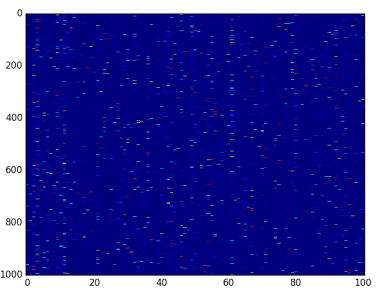
\includegraphics[width=\textwidth]{./fig/conf_mat_untargeted.png}
        \caption{Our speaker classifier's softmax distribution of 1000 samples 
        on approximately 100 speakers.}
        \label{fig:cm_untargeted}
    \end{subfigure}
    \qquad
    \begin{subfigure}[b]{0.4\textwidth}
        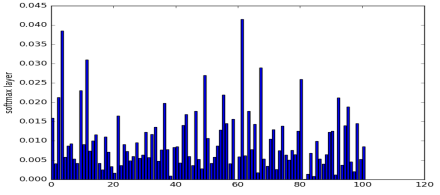
\includegraphics[width=\textwidth]{./fig/histogram_untargeted.png}
        \caption{Our speaker classifier's distribution of randomly sampled 
        speech from the generative model.}
        \label{fig:histogram_untargeted}
    \end{subfigure}
    \qquad
    \begin{subfigure}[b]{0.3\textwidth}
        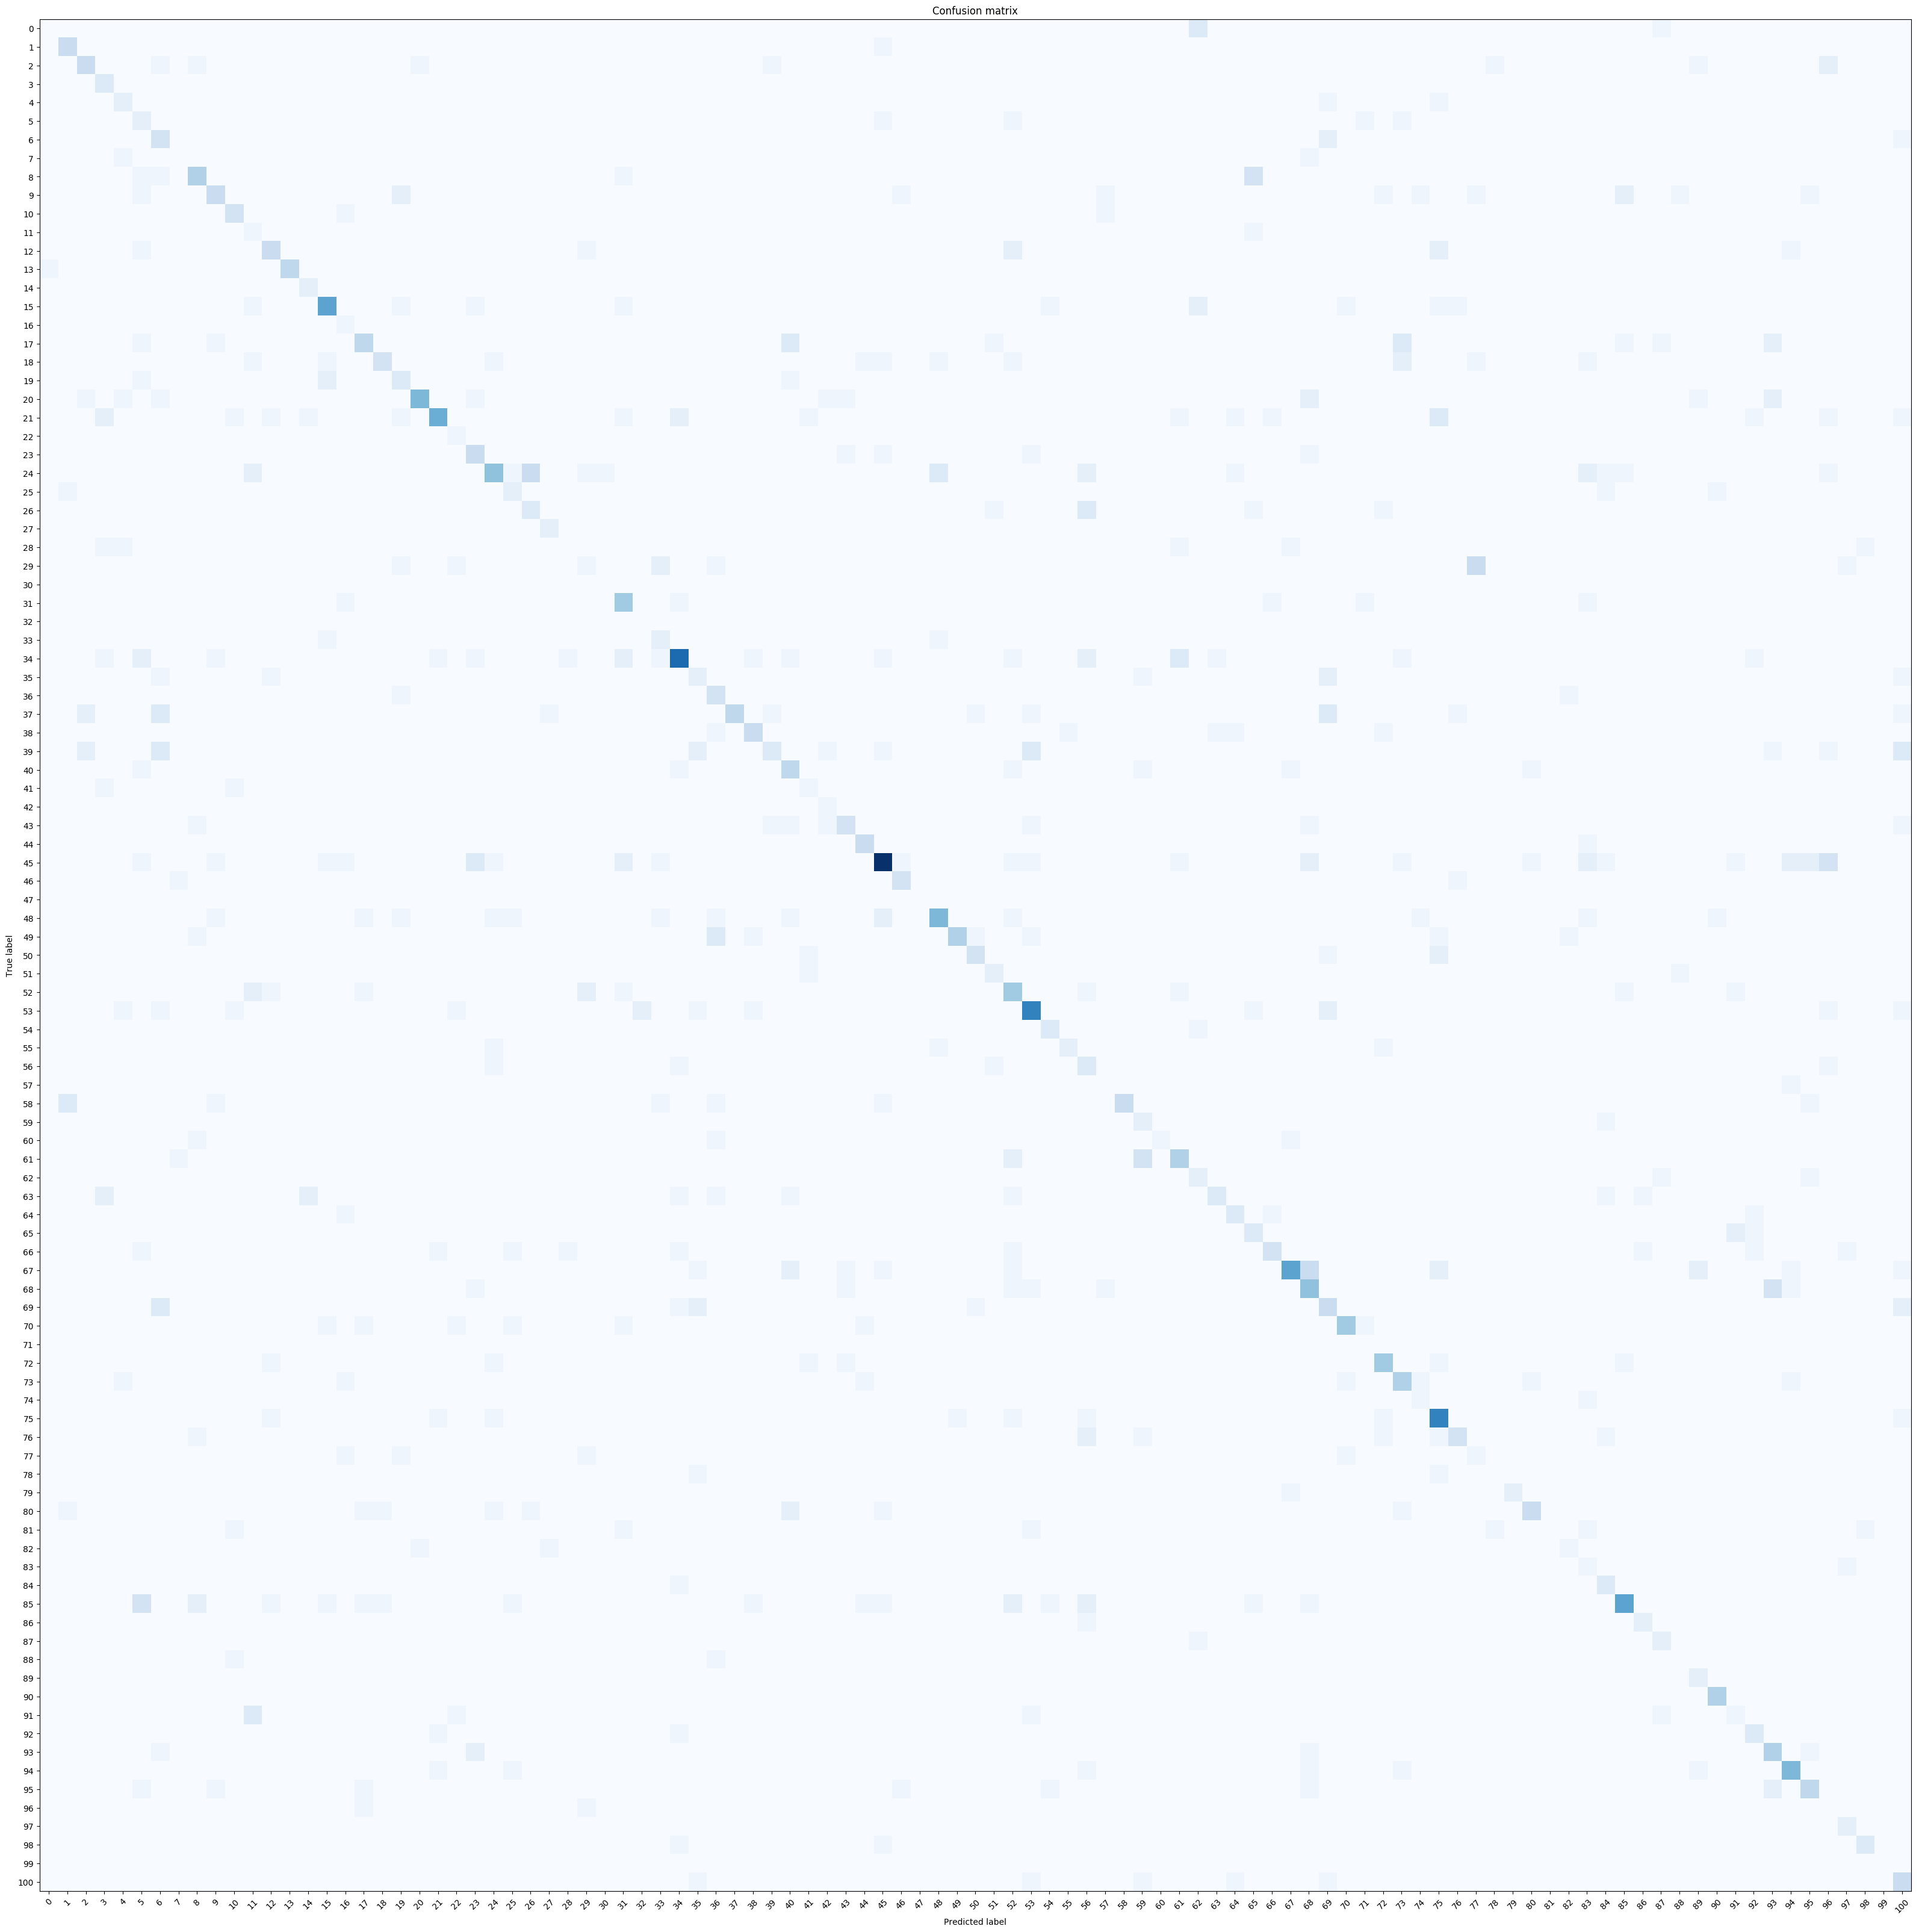
\includegraphics[width=\textwidth]{./fig/conf_mat_cnn_knn.png}
        \caption{Confusion matrix of untargeted model. x-axis corresponds to predicted label, y-axis to ground truth.}
        \label{fig:histogram_untargeted}
    \end{subfigure}
    \caption{Summary of untargeted attacks. Red represents high confidence.}
    \label{fig:conf_mat_cnn_knn}
\end{figure}

As we described earlier, the models for targeted attacks can be trained in two manners: 1) 
conditioning the model on additional information, e.g. class labels, as
described in~\cite{mirza2014conditional}; 2) using only data from the label 
of interest. While the first approach might result in mode collapse, a drawback
of the second approach is that the discriminator, and by consequence the
generator, does not have access to universal\footnote{We draw a parallel with 
Universal Background Models in speech.} properties of speech. In the targeted 
attacks subsection \ref{sub:targeted} we show results using our a new objective function that allows 
using data from all speakers.  

\subsubsection{Untargeted attacks}
\label{sub:untargeted}
For each speaker audio data in the test set, we compute a Mel-Spectrogram as
descibred in section \ref{sub:processdata}. The resulting Mel-Spectrogram is
then fed into the CNN recognizer and we extract a 505-dimensional feature $G$ from
the penultimate fully-connected layer (L7) in the pre-trained CNN model
(\ref{fig:CNN}) trained on the train partition of the real speech dataset with all 
speaker IDs.  This deep feature/embedding $G$ is then used to train a 
K-nearest-neighbor (KNN) classifier, with K equal to 5.

To control the generator trained by our WGAN, we feed the generated
Mel-Spectrograms into the same CNN-L2 pipeline to extract their corresponding
feature $\widehat G$. Utilizing the pre-trained KNN, each sample is assigned to
the nearest speaker in the deep feature space. Therefore, we know which speaker
our generated sample belongs to when we attack our CNN recognizer. We evaluate our
controlled WGAN samples against the state-of-the-art CNN recognizer, and the
confusion matrix can be found in Figure \ref{fig:conf_mat_cnn_knn}. 


\subsubsection{Targeted attacks}
\label{sub:targeted}
We ran all three models (WGAN-GP, SampleRNN, WaveNet) on a mixed corpus containing the entirety of the NIST 2004 corpus, a single speaker (280) from the VCTK Corpus, and the single speaker from the Blizzard dataset. The mixed corpus therefore contains 102 speakers. Samples were created from WaveNet globally conditioned on the single VCTK corpus speaker, and on SampleRNN trained only on data from the Blizzard dataset.
Results are demonstrated in Figure
\ref{fig:confusion_matrices}. Neither WaveNet samples nor sampleRNN samples
were able to attack the recognition model in the same way. In both models, \textbf{none} of the predictions made by the classifier match the target speaker. \\ We also trained the WGAN-GP with mixed loss/without mixed loss on speaker 0. The histogram of predictions in Figure
~\ref{fig:pred_comp_spk0} shows that using the mixed loss model, most of the energy is concentrated on the target speaker 0. The improved WGAN-GP loss achieves 0.38 error
rate and our mixed loss achieves 0.12 error rate, producing a 75\%
increase in accuracy. It is therefore clear that the WGAN-GP mixed loss framework is an improvement on the original loss function, which is expected given the network's access to additional speaker data.

\begin{figure}[t]
    \centering
    \begin{subfigure}[b]{0.3\textwidth}
        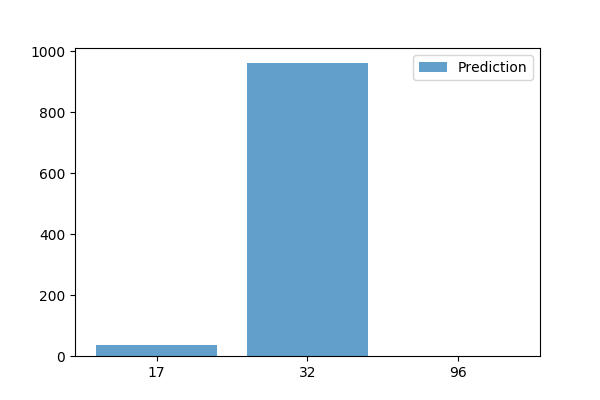
\includegraphics[width=\textwidth]{./fig/pred_histogram_cathy.png}
        \caption{Histogram of sampleRNN predictions. \textbf{Ground truth label: 100}.}
        \label{fig:pred_sampleRNN}
    \end{subfigure}
    \quad
    \begin{subfigure}[b]{0.3\textwidth}
        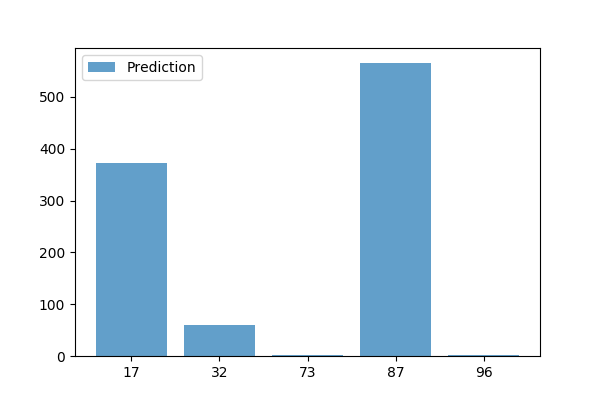
\includegraphics[width=\textwidth]{./fig/pred_histogram_p280.png}
        \caption{Histogram of WaveNet predictions. \textbf{Ground truth label: 101}.}
        \label{fig:pred_wavenet}
    \end{subfigure}
    \quad
    \begin{subfigure}[b]{0.4\textwidth}
        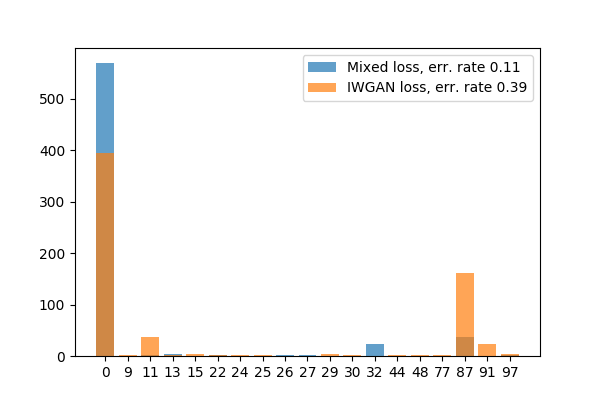
\includegraphics[width=\textwidth]{./fig/pred_comparisson_spk0.png}
        \caption{Histogram of predictions given improved WGAN and mixed loss models.}
        \label{fig:pred_comp_spk0}
    \end{subfigure}
    \caption{Summary histograms of targeted attacks}
    \label{fig:confusion_matrices}
\end{figure}

%
\section{DISCUSSION AND CONCLUSION}\label{sec:conclusions}
In this research we have investigated the use of speech generative models to
perform adversarial attacks on speaker recognition systems. We show that the
samples from autoregressive models we trained, i.e. SampleRNN and WaveNet, or
downloaded from the web were not able to fool the CNN speaker recognizers we
used in this research. On the other hand, we show that adversarial examples
generated with GAN networks are successful in performing targeted and untargeted
adversarial attacks given the speaker recognition used herein.

%
\vfill\pagebreak


\bibliographystyle{IEEEbib}
\bibliography{references}

\end{document}
